\section{评审一致性分析}

% 注：文档主文件需加载 \usepackage{graphicx}（以及可选的 \usepackage{subcaption}）。

\subsection{一致性度量与符号约定}
为衡量不同评审者（judge）对排序结果的一致性，本文基于 \texttt{analysis\_summary\_3d.csv} 在每个评价维度内分别计算 Kendall’s $W$（coefficient of concordance）与评审者两两 Spearman 等级相关系数，并对后者的分布进行统计汇总。

在固定维度下，设共有 $n$ 个候选项（item）与 $m$ 名评审者。候选项索引 $i=1,\dots,n$，评审者索引 $j=1,\dots,m$。令 $r_{ij}$ 表示评审者 $j$ 对候选项 $i$ 给出的名次（名次越小表示排序越优）。

\textbf{Kendall’s $W$（协调系数）}
\begin{equation}
W = \frac{12\,S}{m^2\,(n^3-n)}
\end{equation}
其中
\begin{equation}
S=\sum_{i=1}^{n}(R_i-\bar{R})^2,\quad R_i=\sum_{j=1}^{m} r_{ij},\quad \bar{R}=\frac{1}{n}\sum_{i=1}^{n}R_i.
\end{equation}
其中 $R_i$ 为候选项 $i$ 的“名次和”，$\bar{R}$ 为其均值，$S$ 刻画各候选项名次和的离散程度。$W\in[0,1]$，$W=1$ 表示完全一致，$W\approx 0$ 表示一致性较弱。

\textbf{两两 Spearman 等级相关系数}
对任意两名评审者 $j$ 与 $k$，其排名向量分别记为 $\mathbf{r}_j$ 与 $\mathbf{r}_k$。Spearman 相关系数可表示为名次向量上的 Pearson 相关：
\begin{equation}
\rho_{jk}=\mathrm{corr}(\mathbf{r}_j,\mathbf{r}_k).
\end{equation}
当两位评审者排序趋势一致时，$\rho_{jk}$ 接近 $1$；当排序趋势相反时，$\rho_{jk}$ 接近 $-1$。本文在每个维度内计算全部评审者两两 $\rho_{jk}$，并汇总其均值、中位数以及最小/最大值，以刻画一致性的整体分布。

\subsection{实验结果与统计汇总}
在三个评价维度下计算得到的 Kendall’s $W$ 与两两 Spearman 分布统计如下（相关可视化见图~\ref{fig:judge-corr-eff}--\ref{fig:judge-spearman-box}）：
\begin{itemize}
	\item \textbf{有效性}：一致性最高，$W=0.955$；Spearman 均值 $0.944$（中位数 $0.944$，最小 $0.904$，最大 $0.991$）。
	\item \textbf{无干扰性}：一致性较高，$W=0.846$；Spearman 均值 $0.808$（中位数 $0.839$，最小 $0.585$，最大 $0.932$）。
	\item \textbf{可部署性}：一致性相对较弱，$W=0.687$；Spearman 均值 $0.609$（中位数 $0.689$，最小 $0.238$，最大 $0.947$）。
\end{itemize}
总体而言，评审者在“有效性”维度上的判断最为一致；而“可部署性”维度的分歧更为显著，提示该维度的判定依据可能更依赖经验与主观权衡。

\begin{figure}[t]
	\centering
	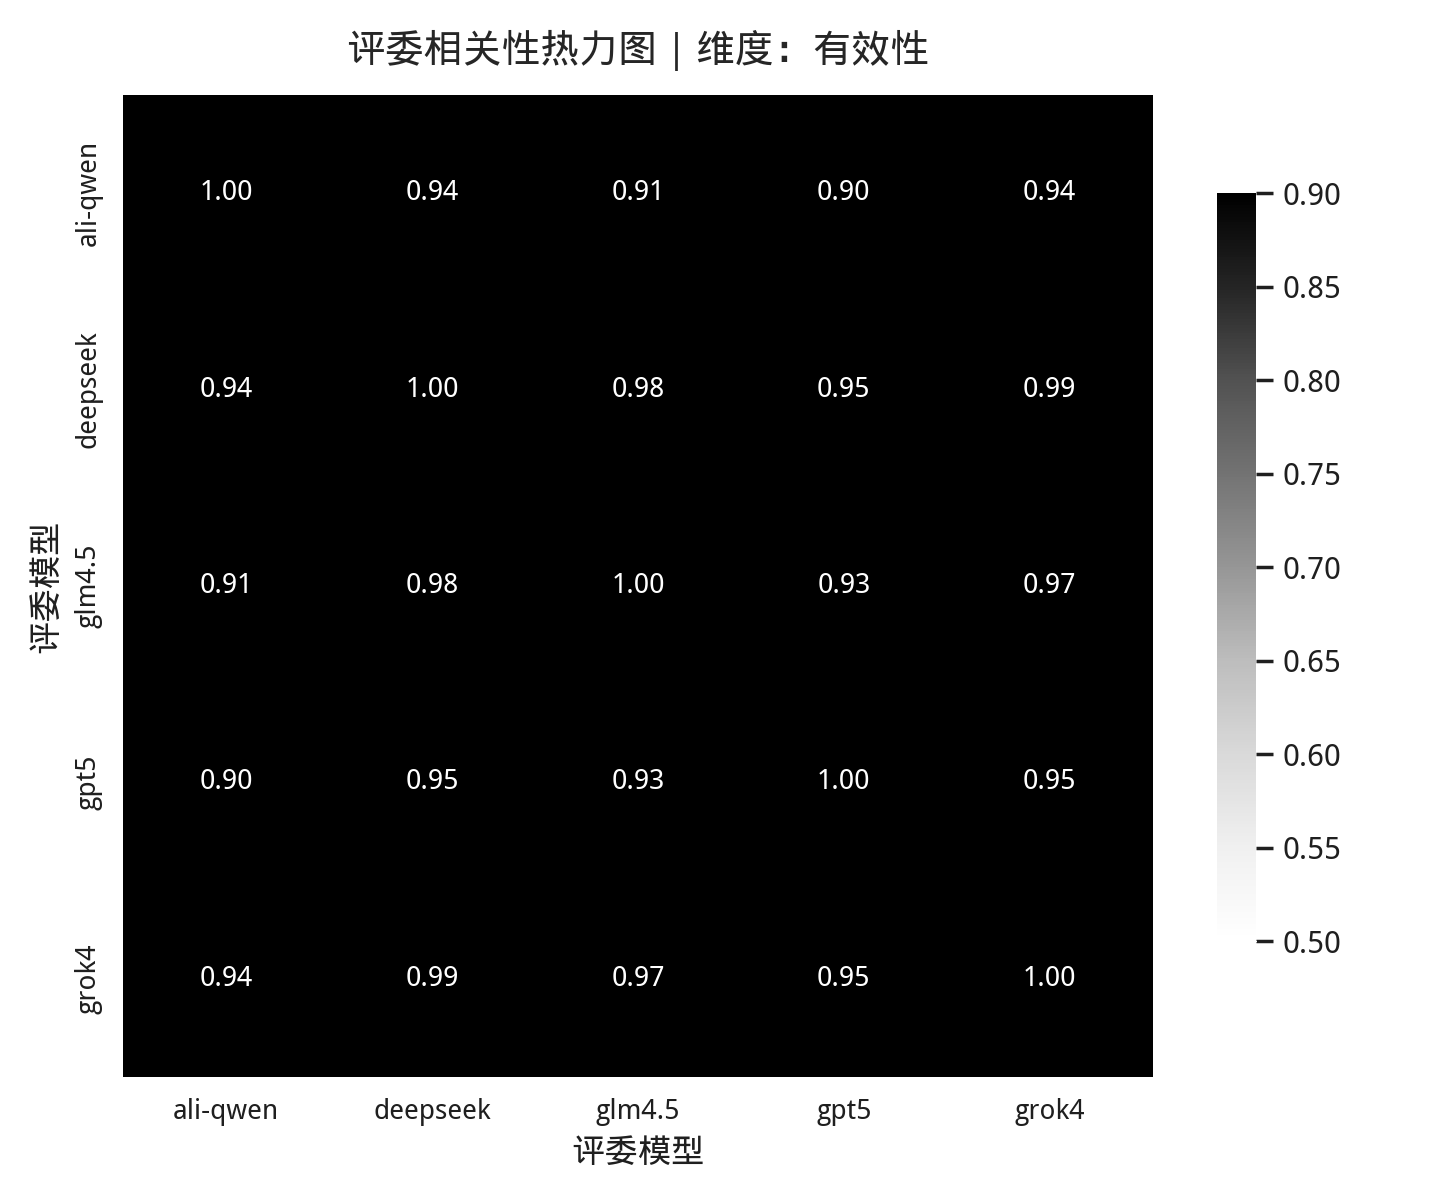
\includegraphics[width=0.86\linewidth]{judge_consistency/judge_correlation_heatmap_有效性.png}
	\caption{有效性维度下评审者两两相关性（Spearman，色标统一；低于阈值区域以白色显示）。}
	\label{fig:judge-corr-eff}
\end{figure}

\begin{figure}[t]
	\centering
	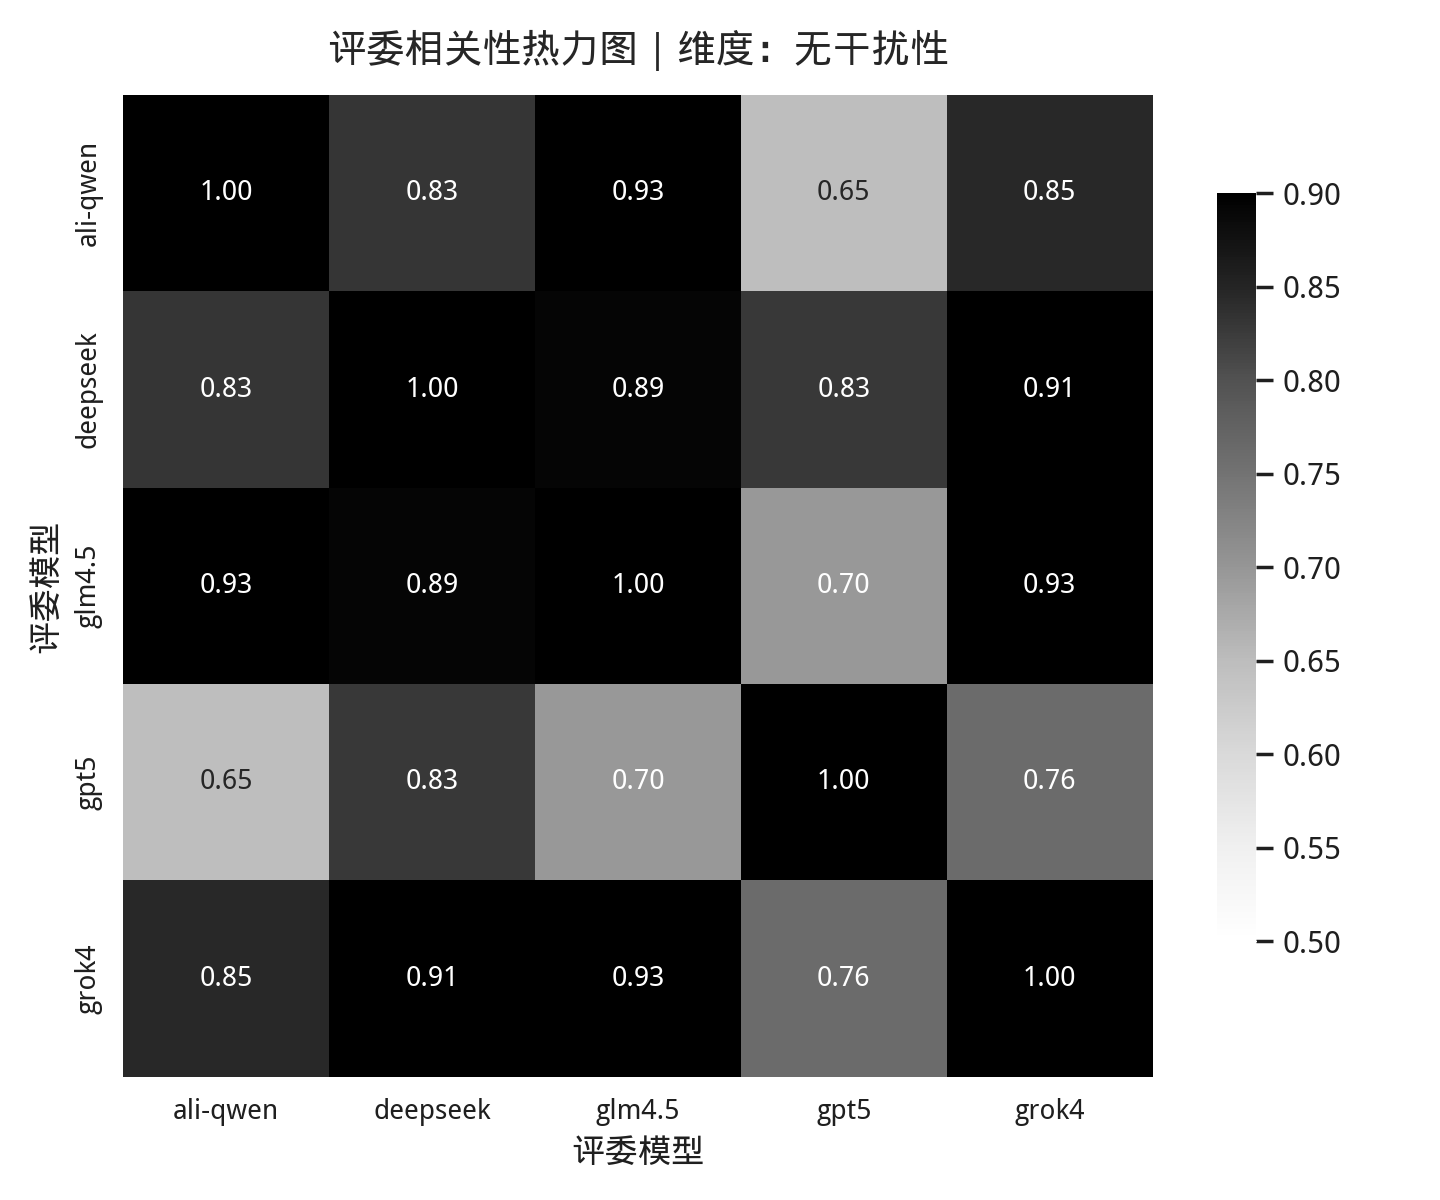
\includegraphics[width=0.86\linewidth]{judge_consistency/judge_correlation_heatmap_无干扰性.png}
	\caption{无干扰性维度下评审者两两相关性（Spearman）。}
	\label{fig:judge-corr-noint}
\end{figure}

\begin{figure}[t]
	\centering
	
\includegraphics[width=0.86\linewidth]{judge_consistency/judge_correlation_heatmap_可部署性.png}
	\caption{可部署性维度下评审者两两相关性（Spearman）。}
	\label{fig:judge-corr-deploy}
\end{figure}

\begin{figure}[t]
	\centering
	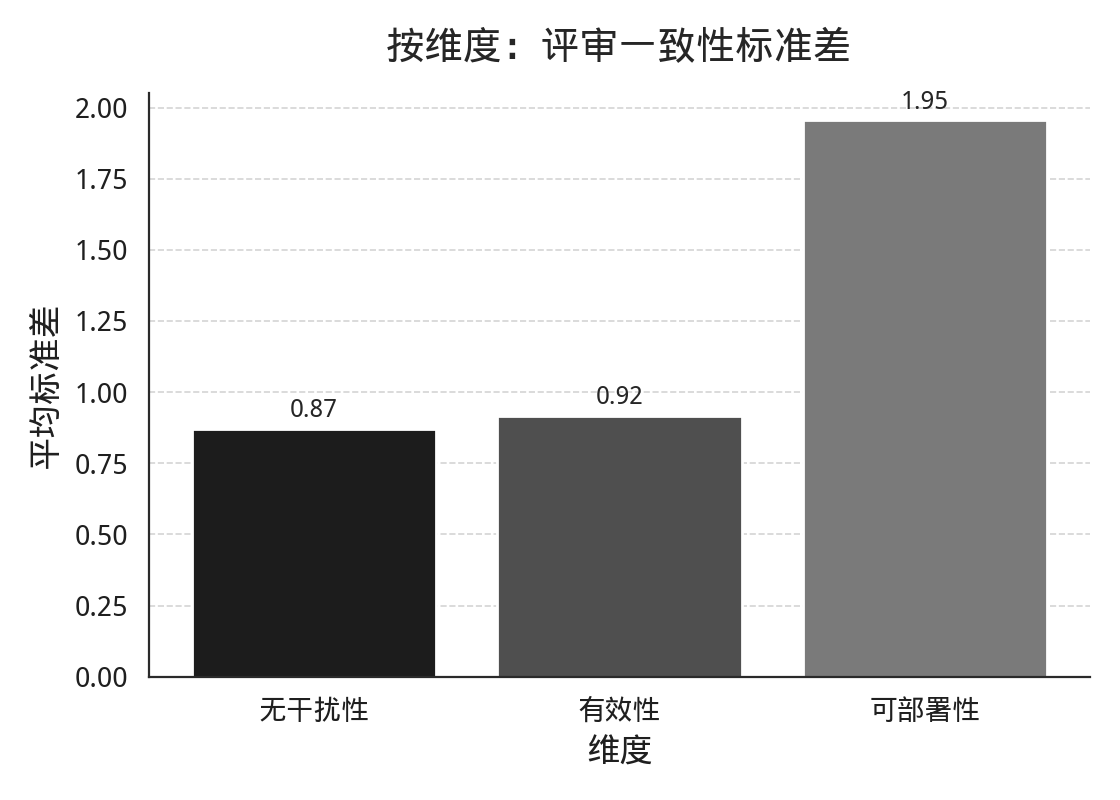
\includegraphics[width=0.86\linewidth]{judge_consistency/judge_dispersion_by_dimension.png}
	\caption{不同维度下评审分歧程度的汇总（以跨评审者的离散性统计量刻画）。}
	\label{fig:judge-dispersion}
\end{figure}

\begin{figure}[t]
	\centering
	
\includegraphics[width=0.86\linewidth]{judge_consistency/judge_kendalls_w_by_dimension.png}
	\caption{各维度 Kendall’s $W$（协调系数）对比。}
	\label{fig:judge-kendalls-w}
\end{figure}

\begin{figure}[t]
	\centering
	
\includegraphics[width=0.86\linewidth]{judge_consistency/judge_spearman_box_by_dimension.png}
	\caption{各维度评审者两两 Spearman 相关系数分布（箱线图）。}
	\label{fig:judge-spearman-box}
\end{figure}

\subsection{讨论与启示}
\textbf{维度差异}：Kendall’s $W$ 与 Spearman 分布呈现一致结论，即“一致性：有效性 $>$ 无干扰性 $>$ 可部署性”。该趋势可由图~\ref{fig:judge-kendalls-w} 与图~\ref{fig:judge-spearman-box} 直观验证；进一步地，相关性热力图（图~\ref{fig:judge-corr-eff}--\ref{fig:judge-corr-deploy}）显示“可部署性”维度中评审者配对相关性的跨度更大。此维度通常涉及工程可行性、环境依赖、部署成本与运维复杂度等多因素综合判断，导致不同评审者的偏好权重与阈值设定存在差异。

\textbf{排序稳定性}：较高的 $W$ 及较高的 Spearman 均值意味着评审者对候选项相对优劣的判断更趋同，从而提升最终排序结果的可解释性与稳定性。相反，当某维度 $W$ 偏低时（见图~\ref{fig:judge-kendalls-w}），应关注排序对评审者选择的敏感性，并结合分歧度汇总图（图~\ref{fig:judge-dispersion}）进一步定位分歧来源，进而细化该维度的评价准则与案例边界。

\textbf{潜在异常评审者效应（可选）}：若两两 Spearman 分布的最小值显著偏低，可能存在与其他评审者系统性差异较大的个体。后续可通过其与其他评审者平均相关度、或对具体分歧样例的定性复核，进一步定位差异来源。
